\chapter{Miscellaneous laboratory tests}\label{appSec:misclab}

In the following section, miscellaneous laboratory performed to strengthen the experimental certainty of the batch sorption isotherm tests are presented. 

\subsection{pH and conductivity}

\begin{figure} 
\centering
\caption{Plot of pH measurements for 50 mL milli-Q water batch tests with 0.1 g biochars (CWC, ULS, BRL) and 5 g soil (S) (n=3).}
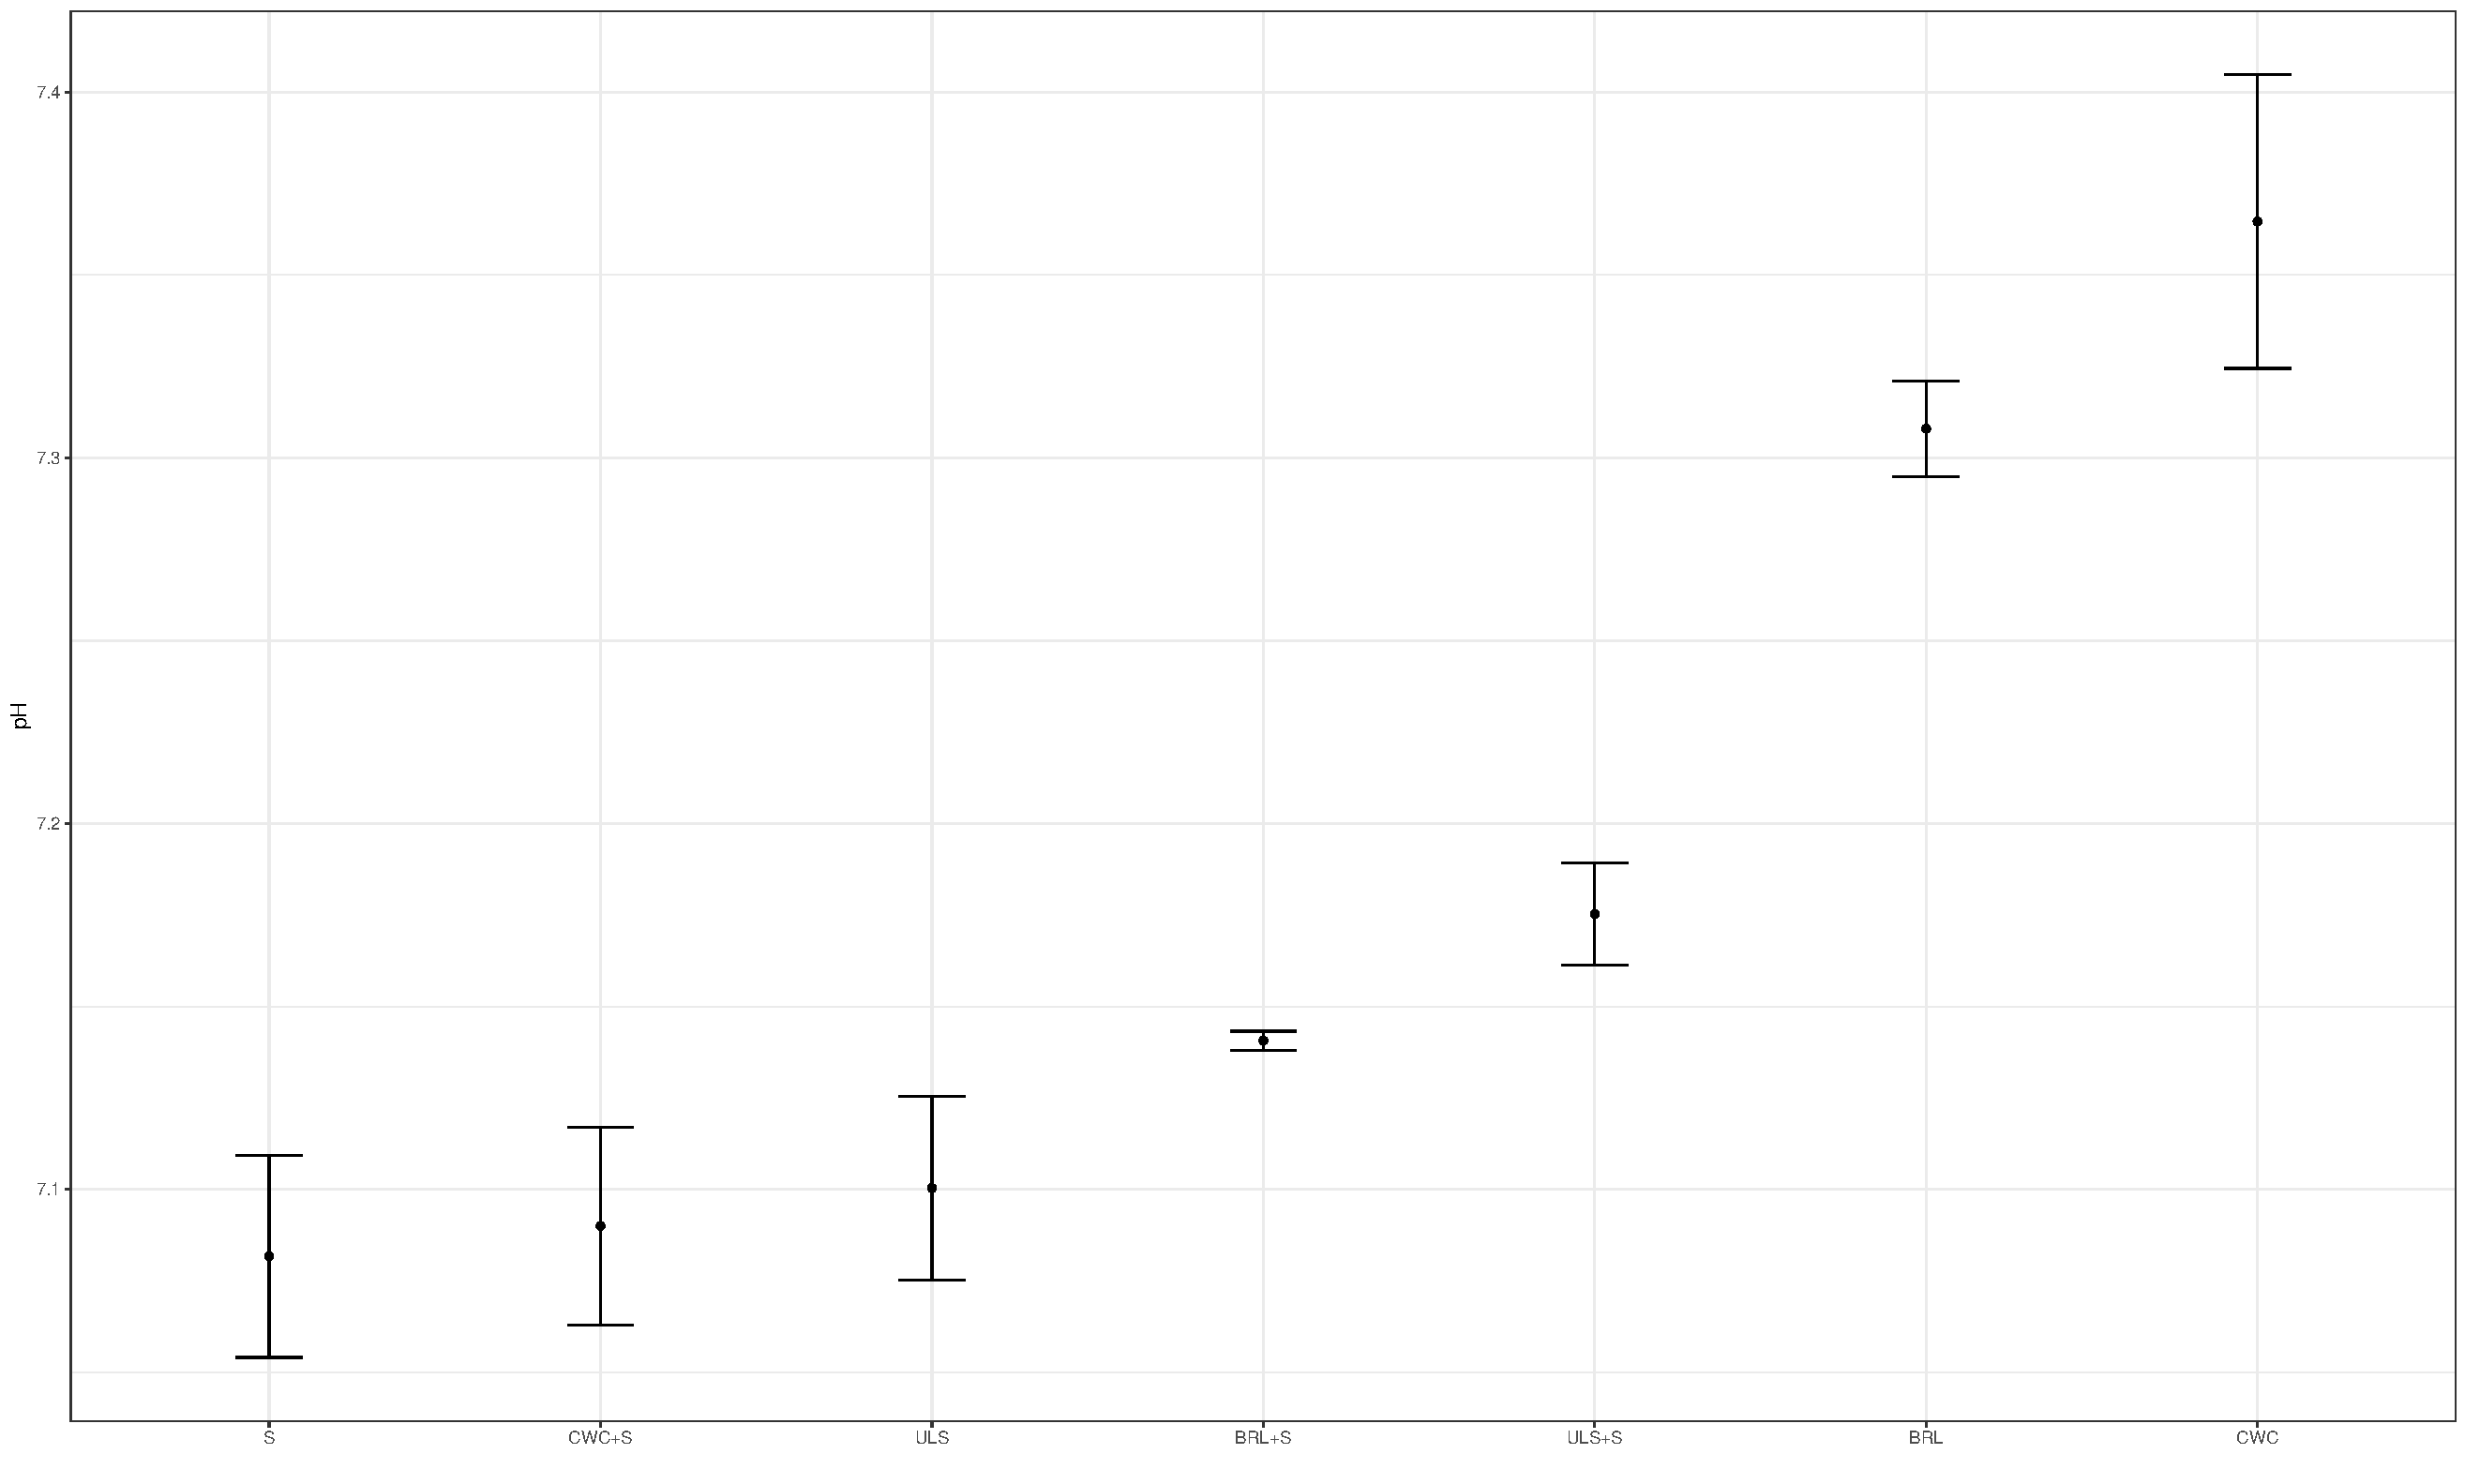
\includegraphics[width=\textwidth]{R/figs/pH.pdf}
\label{appfig:pH}
\end{figure}

\begin{figure} 
\centering
\caption{Plot of conductivity measurements for 50 mL milli-Q water batch tests with 0.1 g biochars (CWC, ULS, BRL) and 5 g soil (S) (n=3).}
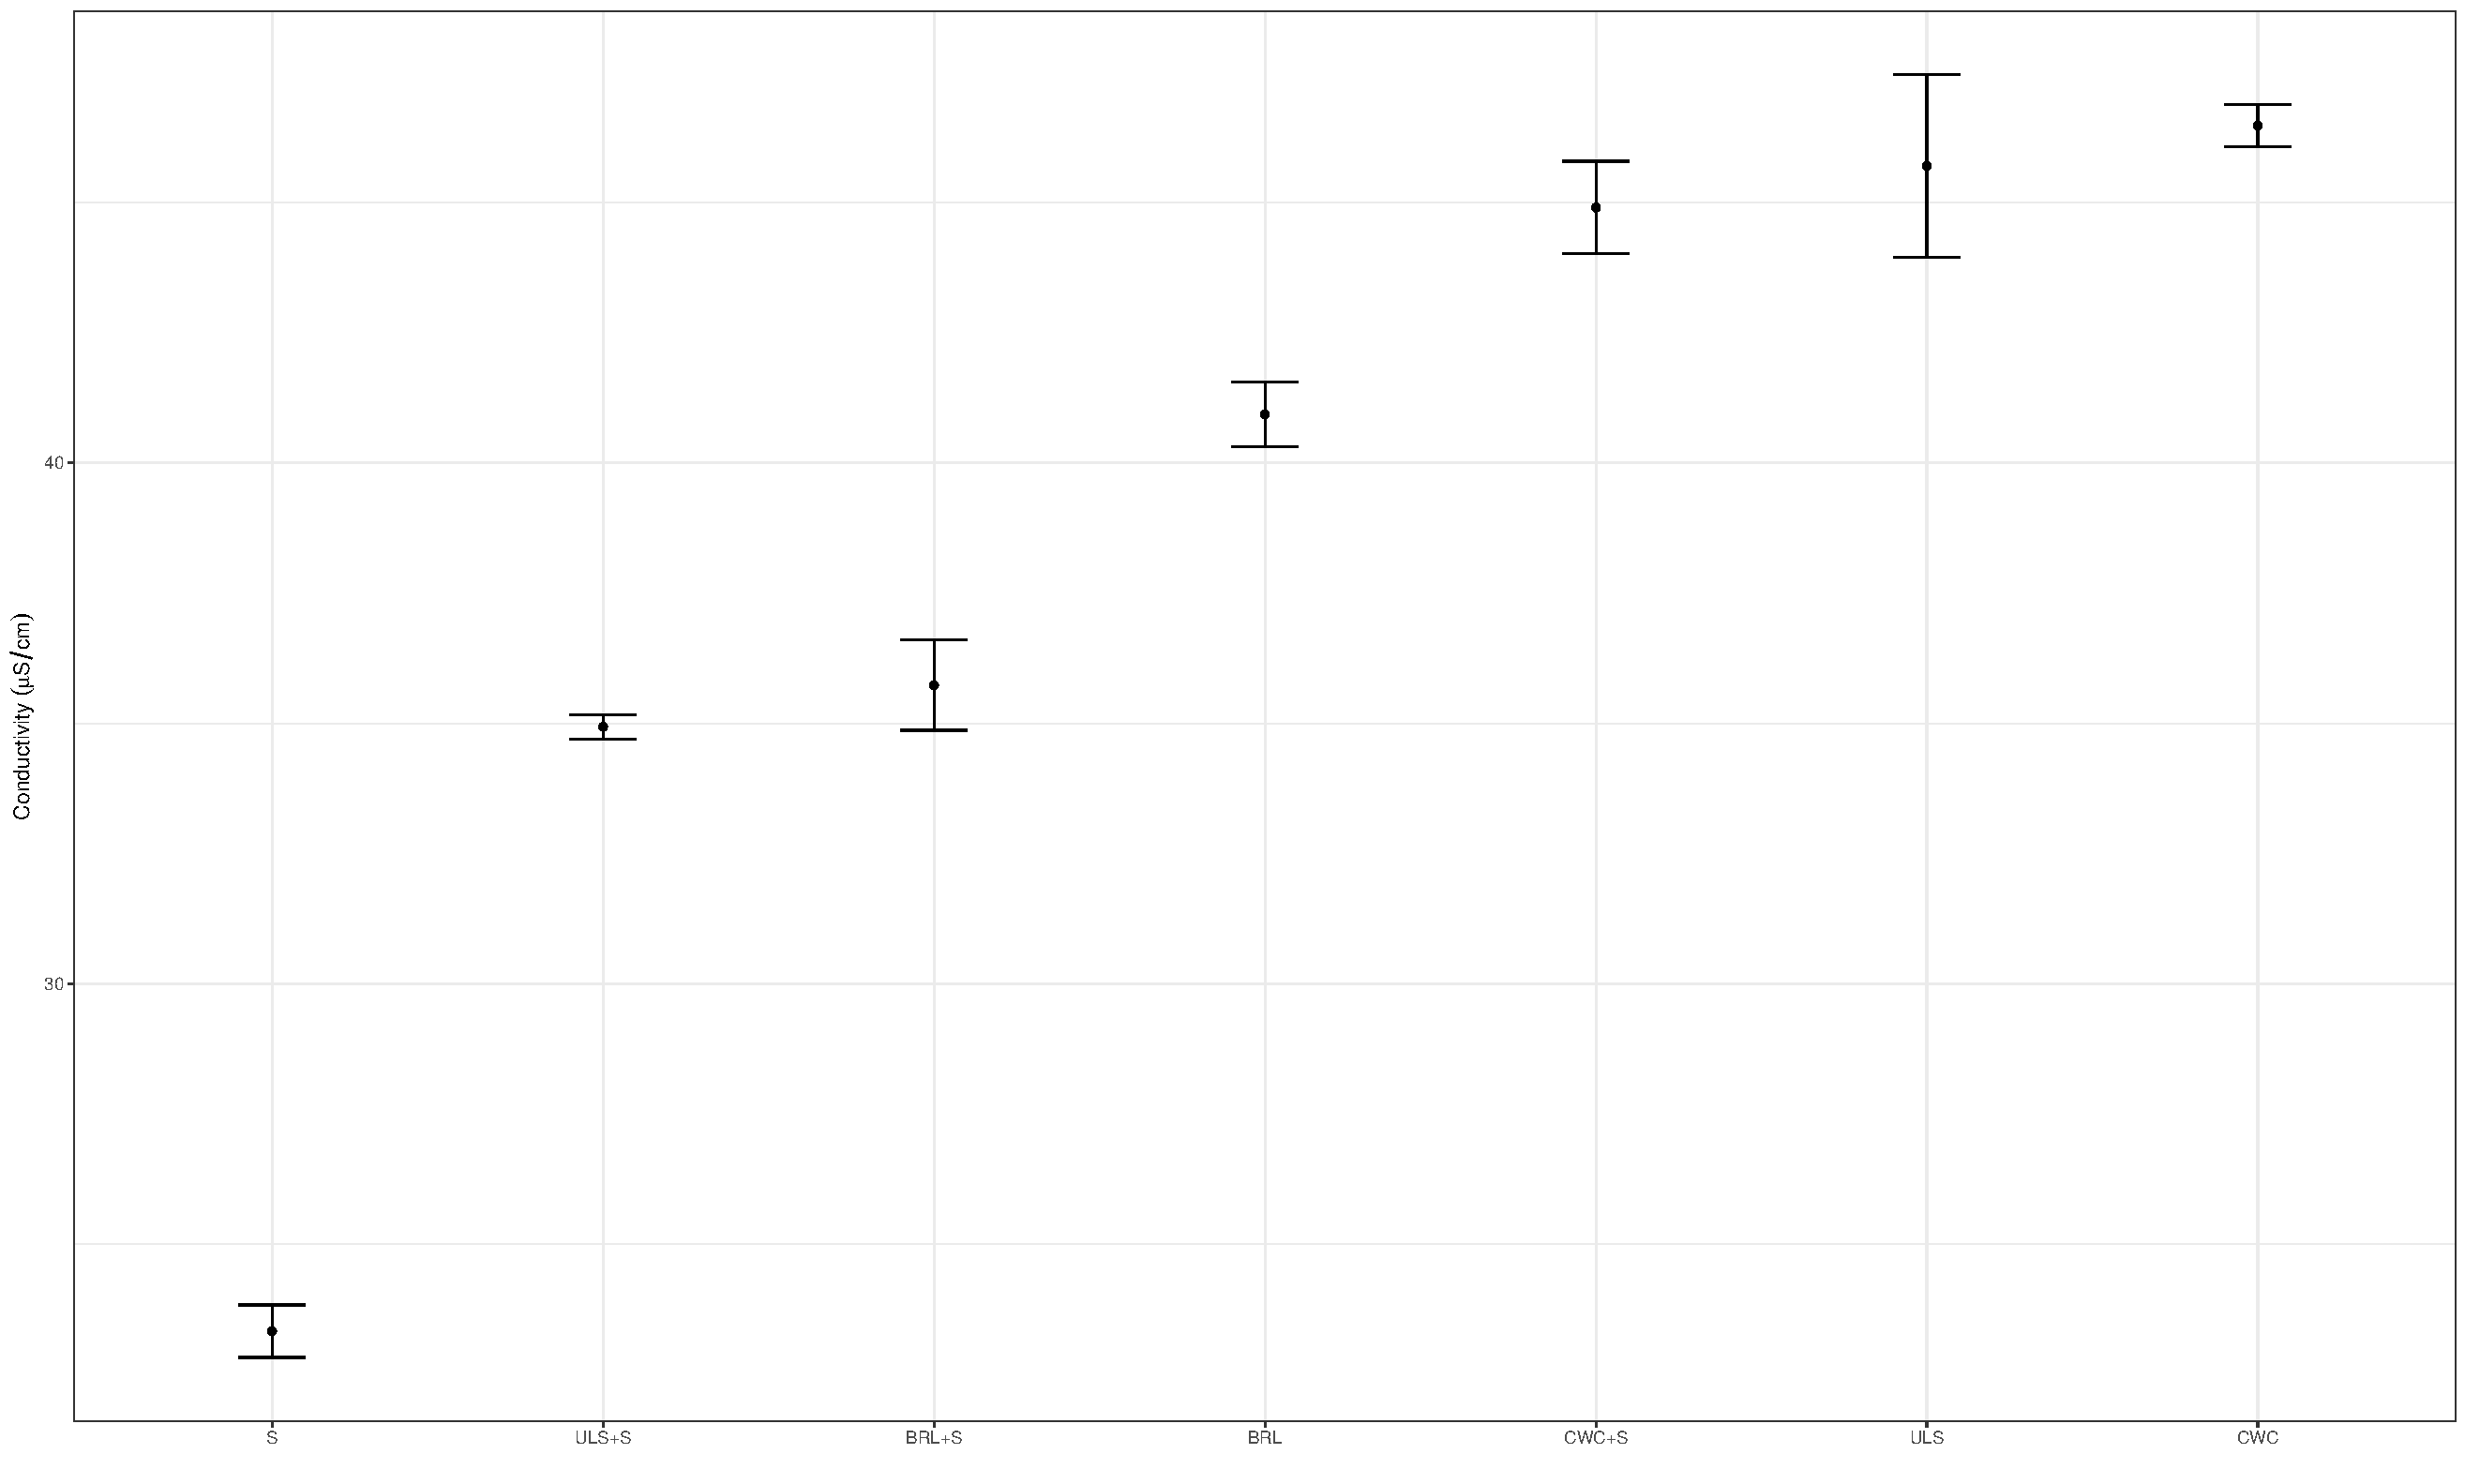
\includegraphics[width=\textwidth]{R/figs/conductivity.pdf}
\label{appfig:cond}
\end{figure}

\begin{table}[h]
\centering
\caption{Pipette calibration for 2-10 mL pipette. PASS is given if CV $\leq$ 1.0 \% and the average volume dispensed is within 1.8400 - 2.1600 mL. }
\label{appTab:pip2-10}
\adjustbox{max width=\textwidth}{%
\begin{tabular}{lrrrrrrr} \toprule
 & \multicolumn{1}{l}{} &  &  &  & \multicolumn{3}{r}{Operator: Thermo Fishcer Scientific} \\
 & \multicolumn{1}{l}{} &  &  &  & \multicolumn{3}{r}{Serial number: EJ08813} \\
 & \multicolumn{1}{l}{} &  &  &  & \multicolumn{3}{r}{Date: 04.10.2021} \\ \midrule
\multicolumn{1}{c}{\textbf{\begin{tabular}[c]{@{}c@{}}Test volume\\ (mL)\end{tabular}}} & \multicolumn{1}{c}{\textbf{}} & \multicolumn{1}{c}{\textbf{\begin{tabular}[c]{@{}c@{}}Weight of\\ dispensed\\ volume (g)\end{tabular}}} & \multicolumn{1}{c}{\textbf{\begin{tabular}[c]{@{}c@{}}Corrected\\ volume (g)\end{tabular}}} & \multicolumn{1}{c}{\textbf{\begin{tabular}[c]{@{}c@{}}Average\\ volume (mL)\end{tabular}}} & \multicolumn{1}{c}{\textbf{SDEV}} & \multicolumn{1}{c}{\textbf{CV}} & \multicolumn{1}{c}{\textbf{PASS/FAIL}} \\ \midrule
\multicolumn{1}{c}{\textbf{2}} & \multicolumn{1}{c}{\textbf{}} &  &  & 2.0868 & 0.006 & 0.3 \% &  \\
\multicolumn{1}{c}{\textbf{}} & 1 & 2.0804 & 2.0842 &  &  &  &  \\
 & 2 & 2.0923 & 2.0961 &  &  &  &  \\
 & 3 & 2.0902 & 2.0940 &  &  &  &  \\
 & 4 & 2.0861 & 2.0899 &  &  &  &  \\
 & 5 & 2.0817 & 2.0855 &  &  &  &  \\
 & 6 & 2.0852 & 2.0890 &  &  &  &  \\
 & 7 & 2.0807 & 2.0845 &  &  &  &  \\
 & 8 & 2.0829 & 2.0867 &  &  &  &  \\
 & 9 & 2.0778 & 2.0815 &  &  &  & \textbf{} \\
 & 10 & 2.0727 & 2.0764 &  &  &  &  \\
 & \multicolumn{1}{l}{} &  &  & \textbf{} & \textbf{} &  & \cellcolor[HTML]{C0C0C0}\textbf{PASS} \\ \bottomrule
\end{tabular}}
\end{table}



\begin{table}
\centering
\caption{Pipette calibration for 200-1000 μL pipette. PASS is given if CV $\leq$ 1.0 \% and the average volume dispensed is within 992 - 1008 μL. }
\label{appTab:pip200-1000}
\adjustbox{max width=\textwidth}{%
\begin{tabular}{lrrrrrrr} \toprule
 & \multicolumn{1}{l}{} & \multicolumn{1}{l}{} & \multicolumn{1}{l}{} & \multicolumn{1}{l}{} & \multicolumn{3}{r}{Operator: Thermo Fischer Scientific} \\
 & \multicolumn{1}{l}{} & \multicolumn{1}{l}{} & \multicolumn{1}{l}{} & \multicolumn{1}{l}{} & \multicolumn{3}{r}{Serial Number: EH23798 4500} \\
 & \multicolumn{1}{l}{} & \multicolumn{1}{l}{} & \multicolumn{1}{l}{} & \multicolumn{1}{l}{} & \multicolumn{3}{r}{Date: 04.10.2021} \\ \midrule
\multicolumn{1}{c}{\textbf{\begin{tabular}[c]{@{}c@{}}Test volume \\ (μL)\end{tabular}}} & \textbf{} & \multicolumn{1}{c}{\textbf{\begin{tabular}[c]{@{}c@{}}Weight of\\ dispensed\\ volume (g)\end{tabular}}} & \multicolumn{1}{c}{\textbf{\begin{tabular}[c]{@{}c@{}}Corrected\\ volume (μL)\end{tabular}}} & \multicolumn{1}{c}{\textbf{\begin{tabular}[c]{@{}c@{}}Average\\ volume (μL)\end{tabular}}} & \multicolumn{1}{c}{\textbf{SDEV}} & \multicolumn{1}{c}{\textbf{CV}} & \multicolumn{1}{c}{\textbf{PASS/FAIL}} \\ \midrule
\multicolumn{1}{c}{\textbf{1000}} & \textbf{} & \multicolumn{1}{l}{} & \multicolumn{1}{l}{} & 994.2 & 5 & 0.5 \% & \multicolumn{1}{l}{} \\
\multicolumn{1}{c}{} & 1 & 997.0 & 998.8 &  &  &  &  \\
 & 2 & 999.4 & 1001.2 &  &  &  &  \\
 & 3 & 990.4 & 992.2 &  &  &  &  \\
 & 4 & 992.3 & 994.1 &  &  &  &  \\
 & 5 & 990.5 & 992.3 &  &  &  &  \\
 & 6 & 990.9 & 992.7 &  &  &  &  \\
 & 7 & 983.8 & 985.6 &  &  &  &  \\
 & 8 & 990.9 & 992.7 &  &  &  &  \\
 & 9 & 990.5 & 992.3 &  &  &  &  \\
 & 10 & 998.4 & 1000.2 &  &  &  &  \\
 & \multicolumn{1}{l}{} & \multicolumn{1}{l}{} & \multicolumn{1}{l}{} & \multicolumn{1}{l}{\textbf{}} & \multicolumn{1}{l}{\textbf{}} & \multicolumn{1}{l}{} & \multicolumn{1}{l}{\cellcolor[HTML]{C0C0C0}\textbf{PASS}} \\ \bottomrule
\end{tabular}}
\end{table}


\begin{table}
\centering
\caption{Pipette calibration for 5 - 50 μL pipette. PASS is given if CV $\leq$ 2.5 \% and the average volume dispensed is within 19.8 - 20.2 μL. }
\label{appTab:pip5-50}
\adjustbox{max width=\textwidth}{%
\begin{tabular}{lrrrrrrr} \toprule
 & \multicolumn{1}{l}{} & \multicolumn{1}{l}{} & \multicolumn{1}{l}{} & \multicolumn{1}{l}{} & \multicolumn{3}{r}{Operator: Thermo Fischer Scientific} \\
 & \multicolumn{1}{l}{} & \multicolumn{1}{l}{} & \multicolumn{1}{l}{} & \multicolumn{1}{l}{} & \multicolumn{3}{r}{Serial Number: EH94947 4500} \\
 & \multicolumn{1}{l}{} & \multicolumn{1}{l}{} & \multicolumn{1}{l}{} & \multicolumn{1}{l}{} & \multicolumn{3}{r}{Date: 04.10.2021} \\ \midrule
\multicolumn{1}{c}{\textbf{\begin{tabular}[c]{@{}c@{}}Test volume\\ (μL)\end{tabular}}} & \multicolumn{1}{c}{\textbf{}} & \multicolumn{1}{c}{\textbf{\begin{tabular}[c]{@{}c@{}}Weight of\\ dispensed\\ volume (g)\end{tabular}}} & \multicolumn{1}{c}{\textbf{\begin{tabular}[c]{@{}c@{}}Corrected\\ volume (mL)\end{tabular}}} & \multicolumn{1}{c}{\textbf{\begin{tabular}[c]{@{}c@{}}Average\\ volume (mL)\end{tabular}}} & \multicolumn{1}{c}{\textbf{SDEV}} & \multicolumn{1}{c}{\textbf{CV}} & \multicolumn{1}{c}{\textbf{PASS/FAIL}} \\ \midrule
\multicolumn{1}{c}{\textbf{20}} & &  &  & 19.8 & 0.4 & 2 $\%$ & \multicolumn{1}{l}{} \\
 & 1 & 19.8 & 19.8 &  &  &  &  \\
 & 2 & 19.5 & 19.5 &  &  &  &  \\
 & 3 & 19.8 & 19.8 &  &  &  &  \\
 & 4 & 20.8 & 20.8 &  &  &  &  \\
 & 5 & 19.9 & 19.9 &  &  &  &  \\
 & 6 & 19.6 & 19.6 &  &  &  &  \\
 & 7 & 19.7 & 19.7 &  &  &  &  \\
 & 8 & 19.5 & 19.5 &  &  &  &  \\
 & 9 & 19.2 & 19.2 &  &  &  &  \\
 & 10 & 19.9 & 19.9 &  &  &  & \cellcolor[HTML]{FFFFFF}\textbf{} \\
 & \multicolumn{1}{l}{} & \multicolumn{1}{l}{} & \multicolumn{1}{l}{} &  &  &  & \multicolumn{1}{l}{\cellcolor[HTML]{C0C0C0}\textbf{PASS}} \\ \bottomrule
\end{tabular}}
\end{table}

\begin{table}
\centering
\caption{Volume calibration for 50 mL Falcon high-clarity polypropylene (PP) conical centrifuge tube. PASS is given if CV $\leq$ and the average volume filled is within 49.0 - 51.0 mL.}
\label{appTab:PPcentrifuge}
\adjustbox{max width=\textwidth}{%
\begin{tabular}{crrrrrrrr} \toprule
 &  &  &  &  & \multicolumn{4}{r}{Date: 26.10.2021} \\ \midrule
\multicolumn{1}{c}{\textbf{\begin{tabular}[c]{@{}c@{}}Test\\volume (mL)\end{tabular}}} & \multicolumn{1}{c}{\textbf{}} & \multicolumn{1}{c}{\textbf{\begin{tabular}[c]{@{}c@{}}Initial \\ weight  (g)\end{tabular}}} & \multicolumn{1}{c}{\textbf{\begin{tabular}[c]{@{}c@{}}Final\\weight (g)\end{tabular}}} & \multicolumn{1}{c}{\textbf{\begin{tabular}[c]{@{}c@{}}Net \\weight (g)\end{tabular}}} & \multicolumn{1}{c}{\textbf{\begin{tabular}[c]{@{}c@{}}Average \\ volume (mL)\end{tabular}}} & \multicolumn{1}{c}{\textbf{SDEV}} & \multicolumn{1}{c}{\textbf{CV}} & \multicolumn{1}{c}{\textbf{PASS/FAIL}} \\ \midrule
\textbf{50} &  &  &  &  & 48.4756 & 0.2 & 0.4 \% &  \\
 & 1 & 13.0354 & 61.3521 & 48.3167 &  &  &  &  \\
 & 2 & 13.0572 & 61.3498 & 48.2926 &  &  &  &  \\
 & 3 & 13.0154 & 61.1161 & 48.1007 &  &  &  &  \\
 & 4 & 13.0857 & 61.8386 & 48.7529 &  &  &  &  \\
 & 5 & 13.0658 & 61.6241 & 48.5583 &  &  &  &  \\
 & 6 & 12.9908 & 61.6972 & 48.7064 &  &  &  &  \\
 & 7 & 13.0073 & 61.4474 & 48.4401 &  &  &  &  \\
 & 8 & 13.0699 & 61.7248 & 48.6549 &  &  &  &  \\
 & 9 & 12.7855 & 61.3788 & 48.5933 &  &  &  &  \\
 & 10 & 12.9962 & 61.3365 & 48.3403 &  &  &  &  \\
 &  &  &  &  &  &  &  & \multicolumn{1}{l}{\cellcolor[HTML]{C0C0C0}\textbf{FAIL}} \\ \bottomrule
\end{tabular}}
\end{table}

\begin{table}
\centering
\caption{Mass CWC left in syringe after filtering of biochar-PFCA solution. Total mass CWC is 0.1000 $\pm$ 0.004 g.}
\label{appTab:CWCloss}
\begin{tabular}{rrrrr} \toprule
 & Mass (g) & \multicolumn{1}{c}{$\bar{x}$} & \multicolumn{1}{c}{SDEV} & \multicolumn{1}{c}{CV}  \\ \midrule
 & & 0.0488 & 0.003 & 8 $\%$ \\
1 & 0.0429 \\
2 & 0.0413 \\
3 & 0.0484 \\
4 & 0.0428 \\
5 & 0.0485 \\ \bottomrule
\end{tabular}
\end{table}

Here can include soil precipitation test?

